\documentclass{boi2014}

\usepackage{enumitem}
\usepackage{todonotes}
\usepackage{wrapfig}

\renewcommand{\DayNum}{2}
\renewcommand{\TaskCode}{demarcation}
\renewcommand{\TaskName}{Demarcation}

\newcommand{\constant}[1]{{\tt #1}}

\begin{document}
    \begin{wrapfigure}{r}{3cm}
        \vspace{-24pt}
		\includegraphics[width=3cm]{\TaskCode.jpeg}
	\end{wrapfigure}

    For a long time the island of Bytopia was ruled by the fair king
    Byteasar. But after the sudden death
    of the king, his two sons---twins Biteon and Byteon---could
    not come to an agreement which one of them should ascend the throne.
    Therefore they decided to divide the island into two provinces to
    rule them independently.  
 
    On a rectangular map Byteotia is shaped as a polygon of $N$ vertices. Every
    side of the polygon is parallel to a side of the map, and every two
    consecutive sides are perpendicular to each other.  Biteon and Byteon want
    to divide the polygon into two congruent figures, using one line segment
    contained in the polygon and parallel to a side of the map.  (Two figures
    are congruent if one can be transformed into the other using a combination
    of reflections, rotations and translations.) Coordinates of the polygon
    vertices and the endpoints of the dividing segment are integers.  
 
    The king's sons asked you to verify whether such a division is
    possible.

    \Task
    Given the shape of the island, determine if it can be partitioned
    by a horizontal or vertical segment into two congruent pieces. If
    it can, find one such segment.
    
    \Input
    The first line of the input contains a single integer $N$, the number of
    vertices. The $i$th of the next $N$ lines contains a pair of integers $X_i$
    and $Y_i$ which are the coordinates of the $i$th vertex.
    The vertices are given in order, i.e. line segments $(X_1,Y_1) - (X_2,Y_2)$,
    $(X_2,Y_2) - (X_3,Y_3)$, \ldots, $(X_{N-1},Y_{N-1}) - (X_N,Y_N)$ and
    $(X_N,Y_N) - (X_1,Y_1)$ are all sides of the polygon.
    Furthermore, any two consecutive line segments in this list are
    perpendicular to each other.

	\Output
	Your program should output a single line. If it is possible to divide the
	island into congruent parts with a horizontal or vertical segment, which
	endpoints are $(x_1, y_1)$ and $(x_2, y_2)$, print 4 integers $x_1$,
	$y_1$, $x_2$ and $y_2$, separated by spaces.
	Either $x_1 = x_2$ or $y_1 = y_2$ must hold.

	If a suitable division cannot be found, output a single word
	\constant{NO}.

    \clearpage

    \Examples
	\example
	{
		10 \newline
		0 0 \newline
		1 0 \newline
		1 1 \newline
		3 1 \newline
		3 5 \newline
		2 5 \newline
		2 3 \newline
		1 3 \newline
		1 2 \newline
		0 2
	}
	{
		1 2 3 2
	}
	{
        Note that there is more than one correct answer in this example.

        \begin{center}
            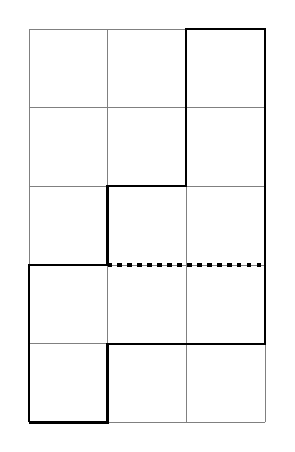
\begin{tikzpicture}
            \draw[help lines] (0,0) grid (3,5);
            \draw[thick] (0,0) -- (1,0) -- (1,1) -- (3,1) -- (3,5) --
                         (2,5) -- (2,3) -- (1,3) -- (1,2) -- (0,2) -- (0,0);
            \draw[ultra thick,dotted] (1,2) -- (3,2);
            \end{tikzpicture}
        \end{center}
    }

    \example
    {
        6 \newline
        0 0 \newline
        1 0 \newline
        1 1 \newline
        2 1 \newline
        2 2 \newline
        0 2
    }
    {
        NO
    }
    {
        In this case there is no way to divide the island into two congruent
        parts.
        \begin{center}
            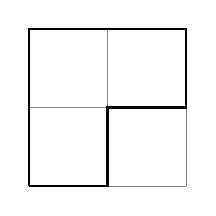
\begin{tikzpicture}
            \draw[help lines] (0,0) grid (2,2);
            \draw[thick] (0,0) -- (1,0) -- (1,1) --
                         (2,1) -- (2,2) -- (0,2) -- (0,0);
            \end{tikzpicture}
        \end{center}
    }

    \Scoring

    \begin{description}
        \item[Subtask 1 (? points).] $4 \le N \le 100\ 000$.
        Any horizontal or vertical line that divides the polygon divides it into
        exactly two parts.
        
        \item[Subtask 2 (? points).] $4 \le N \le 200$.
        \item[Subtask 3 (? points).] $4 \le N \le 4\ 000$.
        \item[Subtask 4 (? points).] $4 \le N \le 100\ 000$.
    \end{description}

    \Constraints

    \begin{description}
        \item[Time limit:] 0.5 s.
        \item[Memory limit:] 256 MB.
    \end{description}

\end{document}
